\documentclass{beamer}
\usetheme{Warsaw}
\usepackage{nhtvslides}
\usepackage{graphicx}
\usepackage{listings}
\lstset{language=CAML,
basicstyle=\ttfamily\footnotesize,
frame=shadowbox,
breaklines=true}
\usepackage[utf8]{inputenc}
\DeclareMathOperator{\sign}{sign}
\DeclareMathOperator{\LookupCurve}{LookupCurve}

\title{Building a physics engine - part 5b: cars}

\author{Dr. Giuseppe Maggiore}

\institute{NHTV University of Applied Sciences \\ 
Breda, Netherlands}

\date{}

\begin{document}
\maketitle

\begin{frame}{Table of contents}
\tableofcontents
\end{frame}

\section{Basic linear dynamics}
\begin{slide}{Basic linear dynamics}{Basic linear dynamics}{
\item Some easy assumptions for starters
\item No gears, lateral forces, etc.
\item Sports car with rear traction
}\end{slide}

\begin{slide}{Basic linear dynamics}{Basic linear dynamics}{
\item Longitudinal force
\begin{eqnarray}
F_{\text{traction}} &=& u F_{\text{engine}} \\
F_{\text{drag}} &=& - C_{\text{drag}} v |v| \\
F_{\text{rr}} &=& - C_{\text{rr}} v \\
F_{\text{long}} &=& F_{\text{traction}} + F_{\text{drag}} + F_{\text{rr}}
\end{eqnarray}
\begin{itemize}
\item $u$ is forward direction
\item $C_{\text{drag}} = 0.4257$
\item $C_{\text{rr}} = 12.8$
\end{itemize}
}\end{slide}

\begin{slide}{Basic linear dynamics}{Basic linear dynamics}{
\item Braking force
\begin{eqnarray}
F_{\text{brake}} &=& -u C_{\text{brake}} \\
F_{\text{long}} &=& F_{\text{brake}} + F_{\text{drag}} + F_{\text{rr}}
\end{eqnarray}
\begin{itemize}
\item $C_{\text{brake}}$ is a constant that \textit{just feels good}
\end{itemize}
}\end{slide}

\section{Weight transfer}
\begin{slide}{Weight transfer}{Weight transfer}{
\item Acceleration causes a pitch of the car
\item It shuffles weight between front and rear
\item Tires with more or less friction, and thus capacity to support acceleration
\item $F_{\text{max}} = \mu W_w$ for a wheel carrying weight $W_w$
\item $\mu \in [1 \dots 1.5]$
}\end{slide}

\begin{frame}{Weight transfer}
\center
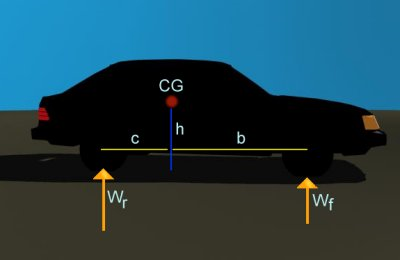
\includegraphics[height=5cm]{Pics/WeightTransfer.png}
\end{frame}

\begin{slide}{Weight transfer}{Weight transfer}{
\item When the car is at rest
\begin{eqnarray}
W_f &=& \frac{c}{l}W \\
W_r &=& \frac{b}{l}W
\end{eqnarray}
\item When the car is accelerating
\begin{eqnarray}
W_f &=& \frac{c}{l}W - \frac{h}{l}ma \\
W_r &=& \frac{b}{l}W + \frac{h}{l}ma
\end{eqnarray}
}\end{slide}

\begin{slide}{Weight transfer}{Weight transfer}{
\item When accelerating, pitch the car
\item If the force applied by the engine to the wheels is bigger than $F_{\text{max}}$, reduce $\mu$ and apply $F_{\text{max}}$, and draw smoke/spinning wheels
\item If the force applied by the engine to the wheels is less than $F_{\text{max}}$, apply the engine force directly
}\end{slide}

\section{Engine force}
\begin{slide}{Engine force}{Engine force}{
\item The engine is not directly connected to the wheels
\item Gears apply the engine torque to different values of max wheel $\tau$ and max wheel $\omega$
\item Lower gears have higher $\tau$
\item Higher gears have higher $\omega$
}\end{slide}

\begin{slide}{Engine force}{Engine force}{
\item $F_{\text{drive}} = u \frac{\tau_{\text{drive}}}{R_w}$ is the force applied to the rear axle
\item $\tau_{\text{drive}} = \tau_{\text{engine}} x_g x_d n$ is the torque applied to the rear axle
\item $\tau_{\text{engine}}$ is the torque coming from the engine given the current RPM
\item $x_g$ is the gear ratio, $x_d$ is the differential ratio
\item $m=1500kg$ is the car mass
\item $n=0.7$ is the transmission efficiency
\item $r_w = 0.34m$ is the wheels radius
}\end{slide}

\begin{slide}{Engine force}{Gear ratios}{
\item $x_g = 2.66\ 1.78\ 1.3\ 1.0\ 0.74\ 0.5$
\item reverse gear $ = 2.9$
\item $x_d = 3.42$
}\end{slide}

\begin{slide}{Engine force}{Torque and RPM}{
\item $rpm$ determines the current maximum torque
\item torque accelerates the wheels
\item wheels determine the next $rpm$
\item $rpm$ is capped; after a while (\textit{red-line}) the engine breaks
\item $\tau_{\text{max}}$ is capped as well; one cap per gear
}\end{slide}

\begin{slide}{Engine force}{Torque and RPM}{
\item Torque and RPM recurrences
\begin{eqnarray}
\tau_{\text{max}} &=& \LookupCurve(rpm) \\
\tau_{\text{engine}} &=& \tau_{\text{max}} \alpha_{\text{throttle}} \\
rpm &=& \max(1000, \frac{\omega_w x_g x_d}{2 \pi})
\end{eqnarray}
}\end{slide}

\begin{slide}{Engine force}{Wheel angular velocity}{
\item For $\LookupCurve$, any reasonable bell-shaped curve (different for each gear) will do
\item Or, copy from the sources of \textit{Marco Monster's - Car Physics for Games} tutorial; they contain some data
}\end{slide}

\begin{frame}{Gear plot}
\center
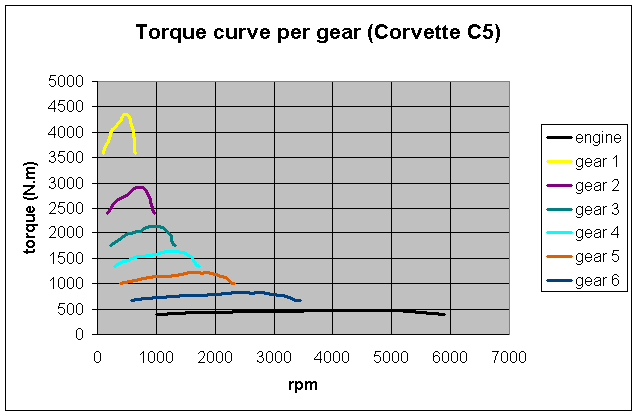
\includegraphics[height=5cm]{Pics/GearPlot.png}
\end{frame}

\begin{slide}{Engine force}{Shifting gears}{
\item RPM changes suddenly when changing gear $rpm' = rpm \frac{x_g'}{x_g}$
}\end{slide}

\begin{slide}{Engine force}{Wheel angular velocity}{
\item Simple solution vs hard solution
\item Simple solution: wheels rotating as car is moving
$$\omega_w \approx \frac{|v|}{r_w}$$
\item Hard solution: track wheel angular velocities separately
}\end{slide}

\section{Slip ratio}
\begin{slide}{Slip ratio}{Slip ratio}{
\item The amount of acceleration of the car depends on the friction between tires and road
\item Rolling tires do not have friction; friction is given by tires rotating faster than they are moving
\item Rear tires roll faster than front tires
}\end{slide}

\begin{frame}{Longitudinal force}
\center
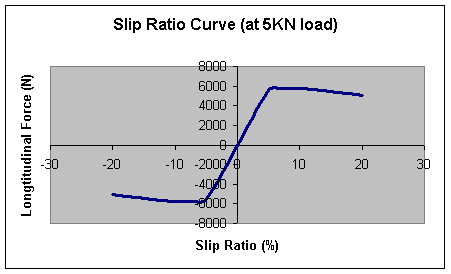
\includegraphics[height=3cm]{Pics/SlipRatioCurve.png}
\end{frame}

\begin{slide}{Slip ratio}{Slip ratio}{
\item Slip ratio determines the force given by the wheel to the car
$\sigma = \frac{\omega_w r_w - v_{\text{long}}}{|v_{\text{long}}|}$
\item The traction force given by the wheel at a certain slip ratio is
$F_{\text{traction}} = \max(6000, C_t \sigma)$
$\tau_{\text{traction}} = F_{\text{traction}} \times R_w$
}\end{slide}

\begin{frame}{Longitudinal force simplified}
\center
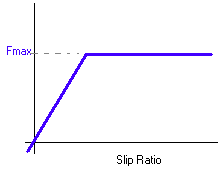
\includegraphics[height=3cm]{Pics/SlipRatioCurveApprox.png}
\end{frame}

\begin{slide}{Slip ratio}{Slip ratio}{
\item We track $\omega_w$ for each wheel
\item We compute the slip ratio and the corresponding torque on the axle
$\tau_{\text{total}} = \tau_{\text{drive}} + \underbrace{\tau_{\text{traction}}}_{\text{two wheels}} + \tau_{\text{brake}}$
\item We compute the angular acceleration of this force on the wheel
$\alpha = \frac{\tau_{\text{total}}}{I_w}$
\item The wheel rotating around its central axis has moment of inertia
$I_w = \frac{m r_w^2}{2}$
}\end{slide}

\section{Curves at a low speed}
\begin{slide}{Curves at a low speed}{Curves at a low speed}{
\item When travelling at low speed
\item We just find the radius of the circle the car describes, depending on the wheel angle
\item $\delta$ is the wheel turn angle
\item $\sin \delta = \frac{L}{R}$
\item From the radius we can determine the angular velocity and just rotate the car by that
$\omega = \frac{v}{R} = \frac{v \sin \delta}{L}$
}\end{slide}

\begin{frame}{Rotation radius}
\center
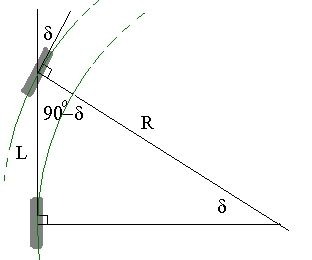
\includegraphics[height=3cm]{Pics/RotationRadius.png}
\end{frame}

\begin{frame}{Delta angle}
\center
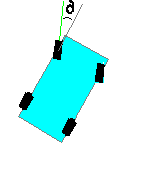
\includegraphics[height=3cm]{Pics/DeltaAngle.png}
\end{frame}

\section{Curves at a high speed}
\begin{slide}{Curves at a high speed}{Curves at a high speed}{
\item Turning the front wheels causes a change in their lateral forces
\item We add new state information to our system
\begin{itemize}
\item $\alpha$ is the side-slip angle of the wheel, which changes as we turn
\item $C_a$ is the cornering stiffness, a pleasant, and utterly fake, constant
\end{itemize}
}\end{slide}

\begin{slide}{Curves at a high speed}{Curves at a high speed}{
\item We compute the lateral and longitudinal speed at a given side-slip angle, for each wheel
\begin{eqnarray}
v_{\text{lat}} &=& |v| \sin \alpha \\
v_{\text{long}} &=& |v| \cos \alpha
\end{eqnarray}
}\end{slide}

\begin{slide}{Curves at a high speed}{Curves at a high speed}{
\item We also compute the side-slip angles given the current angular velocity (started up from low-speed turning) and lateral and longitudinal velocities
\begin{eqnarray}
\alpha_{\text{front}} &=& \frac{v_{\text{lat}} + \omega b}{v_{\text{long}}} - \delta \sign(v_{\text{long}}) \\
\alpha_{\text{rear}} &=& \frac{v_{\text{lat}} - \omega b}{v_{\text{long}}}
\end{eqnarray}
}\end{slide}

\begin{slide}{Curves at a high speed}{Lateral forces}{
\item Lateral force also depends on the current weight distribution 
\item $F_{\text{lateral}} = \max(6000, C_a \alpha) W_w$
\item $\tau_{\text{lateral}} = F_{\text{lateral}} \times b$
\item Each wheel has a different lateral force; we compute torque from lateral forces and use it as usual to further integrate $\omega$
}\end{slide}


\section{Assignment}
\begin{slide}{Assignment}{Assignment}{
\item Before the end of next week
\item Group-work archive/video on Natschool or uploaded somewhere else and linked in your report
\item Individual report by each of you on Natschool
\item Add a personalized selection of forces to your simulator
}\end{slide}

\begin{frame}{That's it}
\center
\fontsize{18pt}{7.2}\selectfont
Thank you!
\end{frame}

\end{document}
